\section{Collecting a GITS Evaluation Set}
\label{sec:challengeset}


While SWE-Agent evaluated their system on SWE-Bench, a collection of open-source repository bugs and their associated fixes, an agent in the Google internal environment would face bugs of a different nature as a result of the environment's idiosyncrasies. To mention a few differences, Google uses a multilingual monorepo~\cite{potvingoogle}, with projects often spanning different portions of the repository, designed to build and run with Google-specific infrastructure (e.g., Bazel~\cite{bazeldistributed}), and with varying levels of domain-specific knowledge required to successfully develop in them. These differences have deep implications for not only writing, running, and testing code, but even for how the agent itself interacts with the Google internal environment (e.g. logging, which is sensitive business data and must be stored accordingly).

GITS, Google's internal issue tracking system, houses a vast and diverse collection of bugs spanning a wide array of projects. This presents both an opportunity and a challenge for automated program repair (APR) systems.
Opportunistically, randomly sampling bugs from GITS may seem appealing, as in principle the full database and constant stream of bugs could benefit from automated repair. 
However, properly selecting sensible bugs is challenging, as ad-hoc random sampling of bugs does not allow for repeatable progress measurement nor does it provide
an informative signal for the potential of APR.

To effectively leverage this resource, we employ a multi-stage filtering funnel to curate a focused set of actionable bugs. This funnel ensures that the bugs presented to Passerine are both relevant to its capabilities and representative of real-world challenges within Google's codebase.
The filtering process comprises four distinct phases, as shown in Figure~\ref{fig:1p-population-curation-diagram}.


\begin{figure}
    \centering
     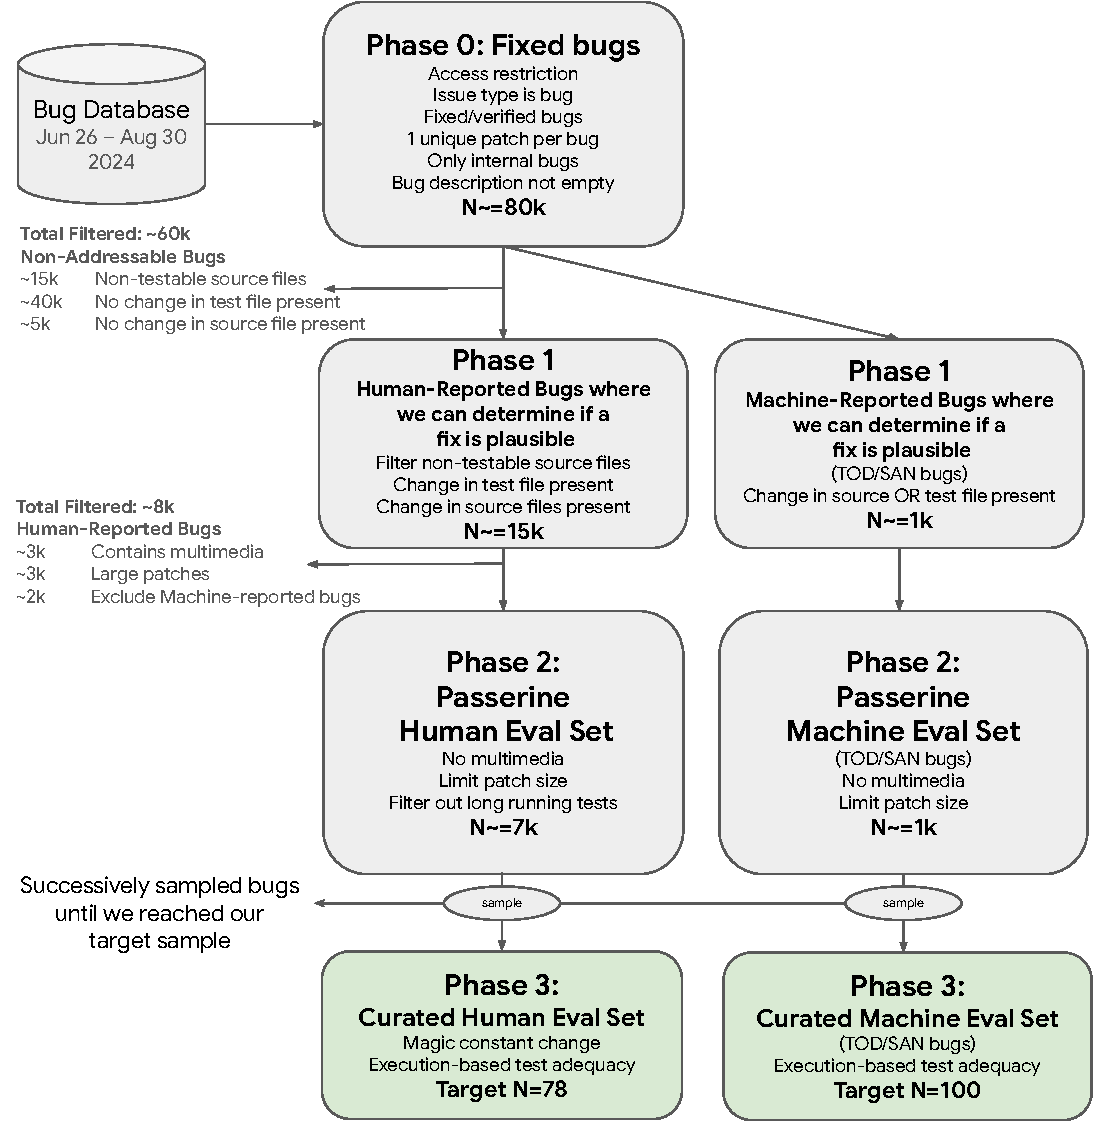
\includegraphics[width=\columnwidth]{figures/bug_filtering_phases.pdf}
    \caption{An overview of the different phases of filtering we go through to collect a GITS evaluation set}
    \label{fig:1p-population-curation-diagram}
\end{figure}


\subsection{Phase 0: Fixed Bugs Population}

This initial phase casts the widest net, aiming to define the broadest possible scope of relevant bugs. We apply minimal filtering criteria (Table~\ref{tab:population-definition-filters}), primarily to ensure accessibility and a clear association between bug reports and their corresponding fixes. This results in a large and diverse initial population of fixed bugs within a specific timeframe, serving as the foundation for further refinement.

\begin{table}[]
\resizebox{\columnwidth}{!}{
    \rowcolors{2}{gray!25}{white}
    \begin{tabular}{ll}
        \rowcolor{gray!50}
    \hline
    Filtering Criteria  & Justification                                                                                                                             \\ \hline
    Access Restriction  & Bug and associated fix must be accessible for analysis.                                                                                   \\
    Issue Type is Bug   & Must be classified as a ``bug'' in our bug database.                                                                                        \\
    Bug Status          & Bug status is ``fixed''.                                                                                                                    \\
    Patch Association   & One bug is associated with one patch, and vice versa.                                                                                     \\
    Bug Description     & Must have a non-empty description                                                                                                         \\
    Project Scope       & \begin{tabular}[c]{@{}l@{}}Restricted to the main Google repository\\
                        (Passerine's current scope).\end{tabular}                                                                     \\
    Bug Source          & Excludes externally reported bugs.                                                                                                         \\
    Patch Data Range    & \begin{tabular}[c]{@{}l@{}}Fix patches are sampled from June 26 to August 30, 2024\\ (chosen for repeatability and to avoid data contamination).\end{tabular} \\
    Bug Creation Cutoff & \begin{tabular}[c]{@{}l@{}}Bugs created no earlier than one year\\
                                before the patch date range start.\end{tabular}                                                                  \\ \hline
    \end{tabular}
}
\caption{Phase 0 
Filters}
\label{tab:population-definition-filters}
\end{table}



\subsection{Phase 1: Bugs Where We Can Determine if a Fix is Plausible
}
Phase 1 refines the selection by focusing on bugs that agentic APR could conceptually address, even if not currently supported by the agent's implementation, and for which we can assess whether the agent generated a plausible fix as part of the evaluation. This necessitates identifying bugs with testable code changes and verifiable fixes. A key aspect of this phase is the separation of human-reported bugs from machine-reported bugs. This distinction allows for tailored filtering criteria based on the nature of the bug report and the availability of information regarding the fix (Table~\ref{tab:phase1-filtering-criteria}).

We focus on two types of machine-reported bugs (Figure~\ref{fig:bug-reports}): those surfaced by the SAN and TOD systems.
SAN performs a variety of sanitizer-based analyses, including memory and thread-related sanitizer reporting, which capture errors such as out-of-bounds accesses, uninitialized values, data races, and more.
Meanwhile, TOD automatically identifies test order-dependence. 

\begin{table}[]
\resizebox{\columnwidth}{!}{
    \begin{tabular}{ll}
    \rowcolor{gray!50}
    \hline
    Filtering Criteria     & Justification                                                                                                                    \\ \hline
    Testable source files  & \begin{tabular}[c]{@{}l@{}}Excludes patches affecting file types that are difficult to \\ test (e.g., sql, html, css, config files).\end{tabular}
    \\ \hline
    \rowcolor{gray!50}
    \multicolumn{2}{l}{Filtering Criteria for Human-Reported Bugs}                                                                                            \\ \hline
    Change in test file    & \begin{tabular}[c]{@{}l@{}}Requires at least one test file to be affected by the patch.\end{tabular}                          \\
    \rowcolor{gray!25}
    Changes in source file & \begin{tabular}[c]{@{}l@{}}Requires at least one source code file (e.g., .cc, .java, .py,\\ .dart, .js, .ts, .go) to be affected by the patch.\end{tabular}
    \\ \hline
    \rowcolor{gray!50}
    \multicolumn{2}{l}{Filtering Criteria for Machine-Reported Bugs}                                                                                          \\ \hline
    Change in code file    & \begin{tabular}[c]{@{}l@{}}The change affects at least a code file that could be either \\ a source code file or a test file.\end{tabular}
    \\ \hline    
    \end{tabular}
}
\caption{Phase 1 Filters}
\label{tab:phase1-filtering-criteria}
\end{table}



\subsection{Phase 2: Automated Curation}
Phase 2 (Table~\ref{tab:phase2-filtering-criteria}) shifts the focus to practical considerations for evaluating our agent's current capabilities. Automated filters are applied to exclude bugs that would pose challenges for evaluation, such as those with long-running integration tests or requiring multi-modal understanding (e.g., screenshots in bug descriptions).

We limit the size of the patch in this phase to be less than 150 lines of code. This number represents the 90th percentile of bug fix patch sizes on a broad set of internal patches, ensuring that we are addressing a wide range of potential bugs.


\begin{table}[]
\resizebox{\columnwidth}{!}{
    \begin{tabular}{llc}
    \rowcolor{gray!50}
    \hline
    Filtering Criteria & Justification & Phase
    
    \\ \hline
    Patch size limit & \begin{tabular}[c]{@{}l@{}}Limits patch sizes to \textless{}150 lines of code for tractability.\end{tabular} & 2      
    \\ \rowcolor{gray!25}
    No multimedia & \begin{tabular}[c]{@{}l@{}}Excludes bugs with multimedia  content in the description.\end{tabular} & 2
    \\
    \begin{tabular}[c]{@{}l@{}}Execution-based \\ Test Adequacy\end{tabular} & \begin{tabular}[c]{@{}l@{}}Confirms that tests associated with the fix reveal the bug, \\ are not flaky, and validate the fix.\end{tabular} & 3                                   
    \\ \rowcolor{gray!25}
    \begin{tabular}[c]{@{}l@{}}No magic constant  \end{tabular} & \begin{tabular}[c]{@{}l@{}}Excludes bugs where fix requires new literals or code symbols\\that cannot be inferred from context.\end{tabular} & 3 \\ \hline                 

    \rowcolor{gray!50}
    \multicolumn{3}{l}{Filtering Criteria for Human-Reported Bugs}                                                                                            \\ \hline
    Long-running tests & \begin{tabular}[c]{@{}l@{}}Excludes bugs with links to our internal integration \\ test platform (likely indicating long test runs).\end{tabular} & 2 \\ \hline
    \end{tabular}
}
\caption{Phase 2 and 3 Filters}
\label{tab:phase2-filtering-criteria}
\end{table}



\subsection{Phase 3: Heuristic Curation}

To begin phase 3, we sample bugs from our phase 2 population and curate them incrementally.
Specifically, we execute any associated test with the
bug and ensure that there are appropriate failures 
before the ground-truth patch, which are then resolved
after the ground-truth patch is applied. In addition, to 
ensure consistent reproducibility, we remove
bugs that exhibit flaky behavior.

Finally, we introduce a layer of human expertise to ensure the quality and relevance of the benchmark set. We conduct manual reviews against a rubric to identify and filter out bugs that are not suited to automatic, execution-based evaluation, such as those relying on ``magic constants'' that cannot currently be easily captured by deterministic automated filters.
We define ``magic constants'' as either literal values (typically strings) or newly introduced code literals (such as method, class, or enum names) that appear in the updated test case but are not present in the original source code. Furthermore, these constants are not readily derivable from the bug report or any other existing code element. This characteristic implies that the successful execution of the bug confirmation test hinges on the precise value of this symbol or constant. However, a valid fix for the underlying bug may not necessitate the exact naming or literal value present in the ground-truth test.
To mitigate the potential for errors in this labeling process, at least one of the authors manually labeled each data point as containing a ``magic constant change'' or not, based on the definition provided above. In cases where the initial annotator was uncertain, a second author reviewed the data point to resolve any ambiguity.  A data point was only labeled as containing a "magic constant change" when both annotators concurred. This negotiated agreement approach helped ensure the reliability of our manual labeling process. 

For the future, we plan to explore automating these heuristics (e.g., through use of few-shot learning given our currently manually labeled set of examples).



This  multi-stage filtering process ensures that the resulting GITS evaluation set (GITS-Eval) is both representative of real-world bugs within Google's codebase and suitable for evaluating the capabilities and potential of agent-based APR. Our final evaluation set comprises 178 bugs: 78 human-reported bugs, and 100 machine-reported bugs, of
which 50 come from automated sanitizers (SAN) and 50 from an automated test order dependency analyzer (TOD). 





\begin{figure}[h]
\vspace{-0.0cm}
    \centering
\begin{adjustbox}{width=0.49\textwidth}
\begin{tabular}{c}
\toprule
\footnotesize{Redacted SAN-reported Bug Report}\\
\midrule
\begin{minipage}[t]{0.45\textwidth}\vspace{-1em}
\begin{lstlisting}[escapeinside=||, breaklines]{text}
|\textbf{Title}|: A REDACTED_SANITIZER_ANALYZER_NAME error (data_race) found while running |\textcolor{red}{REDACTED\_TEST\_TARGET}|
|\textbf{Description}|: We have run |\textcolor{red}{REDACTED\_TEST\_TARGET}| under REDACTED_SANITIZER_ANALYZER_NAME and found one _data_race_ runtime error.

* [Latest run at the time of filing this bug]
(REDACTED_LINK)
* [History of nightly runs of this target]
(REDACTED_LINK)

# How to reproduce this error?
|\textcolor{blue}{REDACTED\_REPRO\_COMMANDS}|
\end{lstlisting}
\end{minipage}\\
\midrule
\footnotesize{Redacted TOD-reported Bug Report}\\
\midrule
\begin{minipage}[t]{0.45\textwidth}\vspace{-1em}
\begin{lstlisting}[escapeinside=||, breaklines=true]{text}
|\textbf{Title}|: Order-dependent test: |\textcolor{red}{REDACTED\_TEST\_TARGET}|
|\textbf{Description}|: ### What's wrong?

REDACTED_ANALYZER_NAME detected order dependence in 
|\textcolor{red}{REDACTED\_TEST\_TARGET}| which means it consistently fails
when running test cases in a particular order.

### How do I reproduce this failure?
|\textcolor{blue}{REDACTED\_REPRO\_COMMANDS}|

### Which test case(s) caused this test to fail?
A simple deductive analysis of randomized test results
shows that |\textcolor{red}{REDACTED\_TEST\_CASE\_1}| always fails when
|\textcolor{red}{REDACTED\_TEST\_CASE\_2}| does not run before it, and always
passes otherwise. Consider whether this test case
affects shared state necessary for |\textcolor{red}{REDACTED\_TEST\_CASE\_1}|
to pass.
\end{lstlisting}
\end{minipage}\\
\bottomrule
\end{tabular}
\end{adjustbox}
\vspace{-0.0cm}
\caption{Machine-reported bug reports, which typically contain richness such as reproduction information.}
\vspace{-0.0cm}
\label{fig:bug-reports}
\end{figure}






\subsection{GITS vs SWE-Bench Bugs}
Understanding the nature of our evaluation set is crucial for interpreting the results of our analysis. To provide context, we compare the distribution of GITS bugs with those in the GitHub-derived SWE-Bench dataset, highlighting important differences in their distributions.
While SWE-Bench does not reflect the entirety of GitHub, it is a widely-used benchmark which sets the standard for evaluating automatic program repair systems.
Thus, to create a comparable test set for GITS, we draw a random sample of 2,000 bug-fixing patches from Phase 1 of our bug filtering phases which comprise both human- and machine-reported bugs for which we can determine a plausible fix. We compare SWE-Bench to Phase 1 bugs, rather than later manually-curated bugs, to capture intrinsic differences in bug distribution without confounding this comparison as a result of Passerine's current limitations (e.g. no multimedia, no flaky tests) or infrastructure challenges (e.g. long running tests).%
This is roughly in line with the methodology used for curation of the SWE-Bench dataset.


We will compare distribution differences along dimensions that correlate with localization difficulty and editing difficulty to highlight the unique challenges Google internal bugs need to address. 


\subsubsection{Localization}

Before a candidate patch can be generated, a fault must be localized to identify what program statements are the root cause for the bug and so should be modified to produce a valid fix. While the difficulty of localization can be influenced by many factors, we consider two aspects: searchability and spatial distribution of changes. 

Code search typically plays a substantial role in localization, as it allows a user to navigate large and potentially unfamiliar codebases~\cite{sadowski2015developers}. Often, code search starts by identifying terms that are relevant to the bug and that may appear in the underlying codebase. To emulate this process, we consider the frequency of terms in a bug issue description that are likely to be codebase symbols, such as class names. We extract these terms using a simple regex-based heuristic, where any term that matches either \texttt{snake\_case} or \texttt{CamelCase} identifiers is considered a code term.
Figure~\ref{fig:rq1-localization-proxy} shows an empirical cumulative distribution function (ECDF) of the number of possible code terms in the associated bug descriptions. We find that GITS bugs have fewer possible code terms in their descriptions.
Only 18\% of GITS bugs have at least 2 possible code terms, compared to approximately 60\% in SWE-Bench.

Next, we consider the extent to which fixes are spatially related. We first compare the number of different files modified by a patch, as well as the number of hunks resulting from the segmentation of those changes~\cite{hunks}. Finally, we also consider patch spread, defined as the number of lines of separation between continuous hunks~\cite{sobreira2018dissection}, as a measure of how much a patch is dispersed throughout a file or across multiple files.
We compute the number of unmodified lines between consecutive changes for each affected file and sum these to yield the patch spread. A higher patch spread suggests a greater degree of interleaving, where modified lines are scattered throughout the file. Conversely, a lower spread indicates that modifications are clustered together in contiguous blocks.


Figures~\ref{fig:spread_files} and~\ref{fig:spread_lines} show that GITS patches modify more files (up to twice as many), and that these modifications result in much larger hunk counts, respectively. When we measure patch spread (Figure~\ref{fig:spread_lines}), we again find that patches are more widely separated within files than those in SWE-Bench.

\begin{figure*}[t!]
    \centering
    \begin{subfigure}[b]{0.19\textwidth}
        \centering
        
\includegraphics[width=\textwidth]{figures/rq1/gits-swe/localization_proxy.pdf}
        \caption{}
        \label{fig:rq1-localization-proxy}
    \end{subfigure}
    \hfill    
    \begin{subfigure}[b]{0.19\textwidth}   
        \centering
        
\includegraphics[width=\textwidth]{figures/rq1/gits-swe/spread_files.pdf}
        \caption{}
        \label{fig:spread_files}
    \end{subfigure}
    \hfill
    \begin{subfigure}[b]{0.19\textwidth}
        \centering
        
\includegraphics[width=\textwidth]{figures/rq1/gits-swe/spread_lines.pdf}
        \caption{}
        \label{fig:spread_lines}
    \end{subfigure}
    \hfill
    \begin{subfigure}[b]{0.19\textwidth}
        \centering
        
\includegraphics[width=\textwidth]{figures/rq1/gits-swe/spread_hunks.pdf}
        \caption{}
        \label{fig:spread_hunks}
    \end{subfigure}
    \hfill
    \begin{subfigure}[b]{0.19\textwidth}
        \centering
        
\includegraphics[width=\textwidth]{figures/rq1/gits-swe/lines_delta_total.pdf}
        \caption{}
        \label{fig:rq1-lines-delta}
    \end{subfigure}    
    \caption{Comparing GITS Phase 1 bugs to SWE-Bench. Changes found in ground-truth patches solving GITS bugs tend to (a) have fewer likely code identifier tokens, which in turn require more sophisticated code search abilities and bug knowledge to successfully localize the original fault. These patches modify substantially more files (b), which are further apart in the codebase (c), and produce changes with many separate hunks (d)
    and more lines of code changed (e).
    }
\end{figure*}

\subsubsection{Editing}

Once a fault location is identified, the associated statements must be edited to produce a fix. Intuitively, larger edits (meaning more lines of code) can pose a challenge as they introduce more opportunities for mistakes. We measured the number of lines changed in ground-truth patches. As shown in Figure~\ref{fig:rq1-lines-delta},
almost all patches from SWE-Bench are under 100 lines while
only
approximately 40\% of GITS patches are under 100 lines.


This complexity is further compounded by the need to consider the specific syntax and semantics of different programming languages. To better understand the language distribution we identified the top 5 most frequent file extensions in our sample of GITS patches (SWE-Bench only considers Python files): Java, C++, TypeScript, Kotlin, and Python.




\vspace{-0.4cm}
\begin{center} 
\fbox{
\begin{minipage}[t]{0.97\linewidth}
{\bf GITS vs SWE-Bench.} 
Our analysis shows that GITS bugs present unique challenges compared to SWE-Bench, particularly in terms of localization and code modification. GITS and SWE-Bench differ slightly in the amount of code-related terms in their descriptions. Additionally, patches for GITS bugs differ in nature when it comes to  changes across files, the number of modified lines, and dispersion of the modifications (i.e., patch spread).
\end{minipage}
}
\end{center}

\subsection{GITS-Eval vs. SWE-Bench-Lite}
We previously introduced GITS-Eval, a more tractable, curated subset of 178 bugs, which we use for evaluation of our agentic repair system.
In an open source context, most state-of-the-art agent-based APR approaches are evaluated on SWE-Bench-Lite, a more practical and self-contained benchmark derived from SWE-Bench. GITS-Eval is the analogous dataset in our context.
Recognizing the potential for variations between human-reported and machine-reported bugs, we have categorized the bugs within GITS-Eval accordingly. 

Figure~\ref{fig:rq1-eval} compares SWE-Bench-Lite, human, and machine-reported
bugs in GITS-Eval. We find that machine-reported bugs in GITS-Eval are comparable to bugs
in SWE-Bench-Lite. Meanwhile, human-reported GITS-Eval bugs display
increased complexity compared to SWE-Bench-Lite, resembling the differences
observed in our earlier comparison of GITS and SWE-Bench.


\begin{figure*}[t!]
    \centering
    \begin{subfigure}[b]{0.19\textwidth}
        \centering
        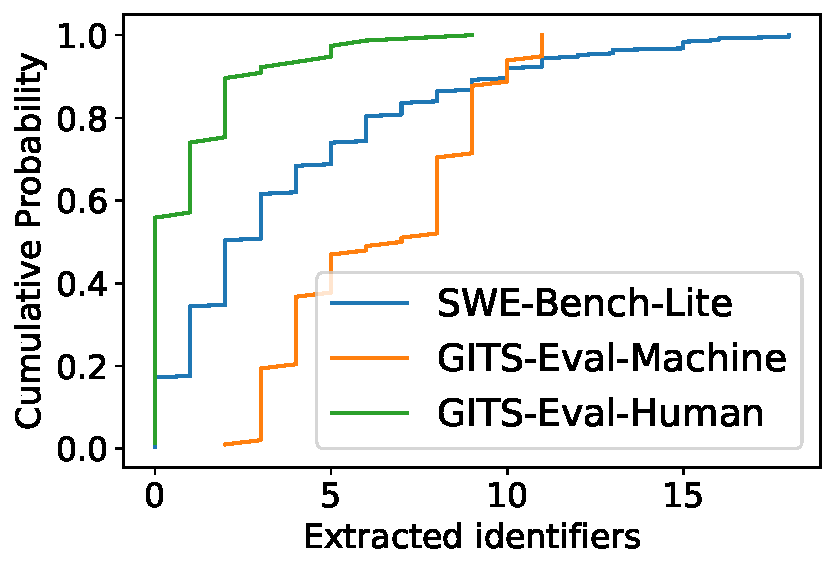
\includegraphics[width=\textwidth]{figures/rq1/gits-swe-lite/localization_proxy.pdf}
        \caption{}
        \label{fig:localization_eval}
    \end{subfigure}
    \hfill    
    \begin{subfigure}[b]{0.19\textwidth}
        \centering
        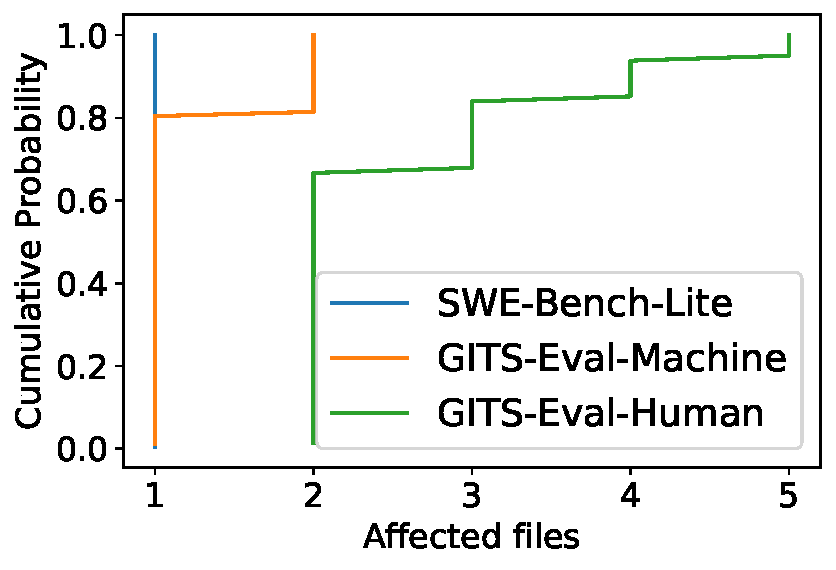
\includegraphics[width=\textwidth]{figures/rq1/gits-swe-lite/spread_files.pdf}
        \caption{}
        \label{fig:spread_files_eval}
    \end{subfigure}
    \hfill
    \begin{subfigure}[b]{0.19\textwidth}
        \centering
        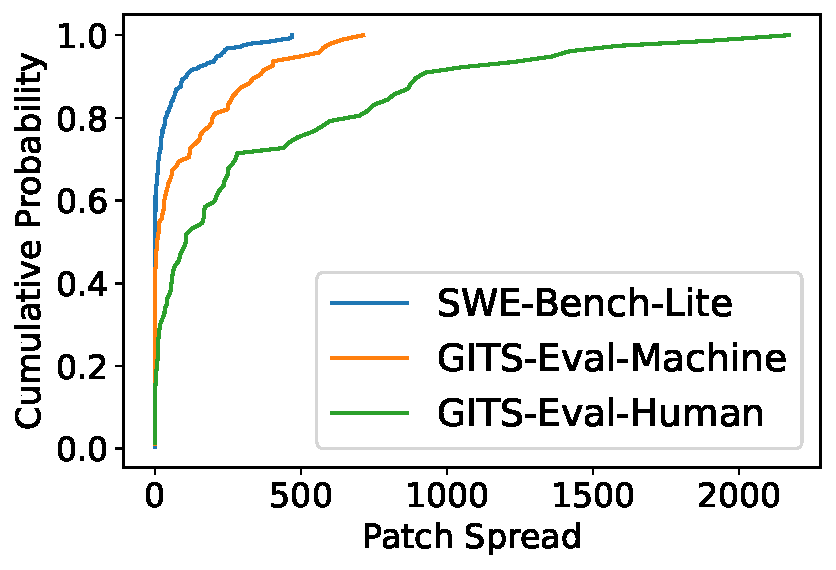
\includegraphics[width=\textwidth]{figures/rq1/gits-swe-lite/spread_lines.pdf}
        \caption{}
        \label{fig:spread_lines_eval}
    \end{subfigure}
    \hfill    
    \begin{subfigure}[b]{0.19\textwidth}
        \centering
        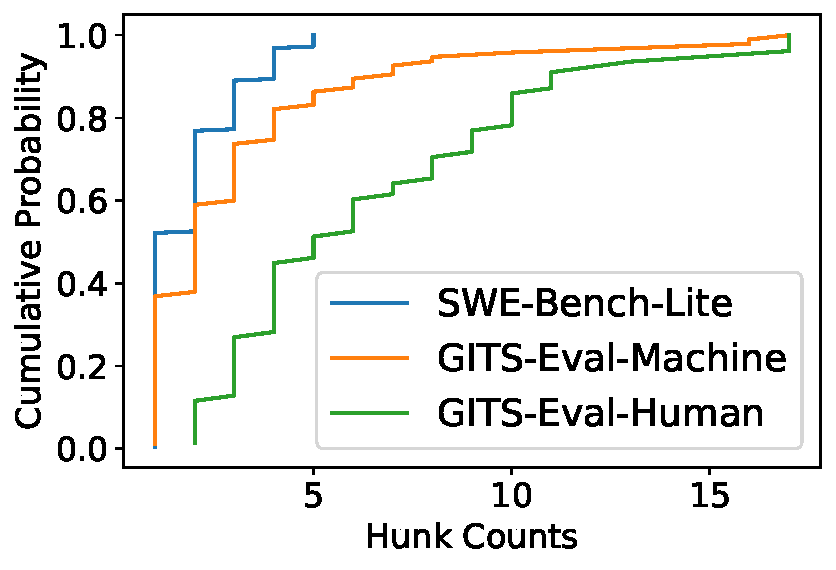
\includegraphics[width=\textwidth]{figures/rq1/gits-swe-lite/spread_hunks.pdf}
        \caption{}
        \label{fig:spread_hunks_eval}
    \end{subfigure}
    \hfill
    \begin{subfigure}[b]{0.19\textwidth}
        \centering
        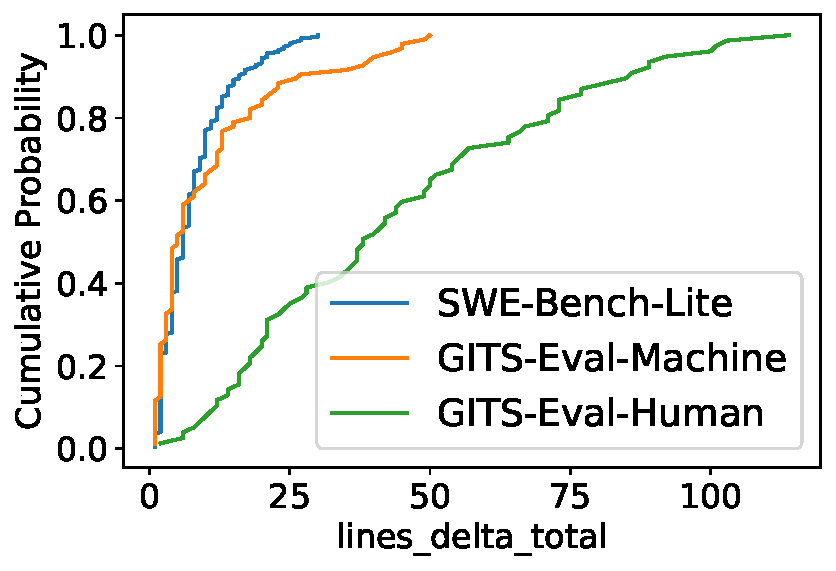
\includegraphics[width=\textwidth]{figures/rq1/gits-swe-lite/lines_delta_total.pdf}
        \caption{}
        \label{fig:rq1-lines-delta_eval}
    \end{subfigure}    
    \caption{
    GITS-Eval machine-reported bugs are comparable to SWE-Bench-Lite, while human-reported 
    GITS-Eval bugs are more complex and resemble differences in our GITS and
    SWE-Bench comparison.
    }
    \label{fig:rq1-eval}
\end{figure*}





